\section{Funzionalit\`a}
\label{section:use-cases}

In questa sezione descriveremo le funzionalit\`a che vogliamo
implementare e, per ognuna di esse, mostreremo i risultati della
realizzazione.

Inoltre, come il lettore capir\`a dalle prossime righe, ogni
funzionalit\`a pu\`o essere messa in corrispondenza con il concetto di
filtro. Quest'associazione porter\`a alla naturale astrazione che
costituir\`a l'architettura della nostra libreria.

\subsection{Costruzione del grafo a partire da una codifica SBML}
L'operazione fondamentale a cui siamo interessati \`e poter manipolare
un modello metabolico, implementando un sistema di oggetti che
permetta di applicare i concetti espressi nel capitolo precedente.

Questa funzionalit\`a \`e necessaria per poter applicare le
successive, in quanto quest'ultime assumono che il modello SBML che si
vuole studiare sia gi\`a rappresentato mediante un grafo.

Non riportiamo nessuna rappresentazione grafica dei risultati di
questa funzionalit\`a in quanto il prodotto \`e un insieme di oggetti
Java che implementano la struttura grafo. Vedremo nella prossima
sezione come sar\`a possibile rappresentarlo graficamente.

\subsection{Rappresentazione grafica del grafo con nodi bianchi e
  neri}
\label{subsection:represent-it-in-black-and-white}
Con questa funzionalit\`a si vuole costruire un documento
interpretabile dai motori di renderizzazione offerti dalla libreria
\emph{graphviz}, rappresentando i nodi sorgenti e nodi pozzi con un
cerchio completamente riempito (\emph{nodi neri}), mentre i nodi che
non sono n\'e sorgenti n\'e pozzi con un cerchio vuoto (\emph{nodi
  bianchi}).
\begin{figure}
  \centering
  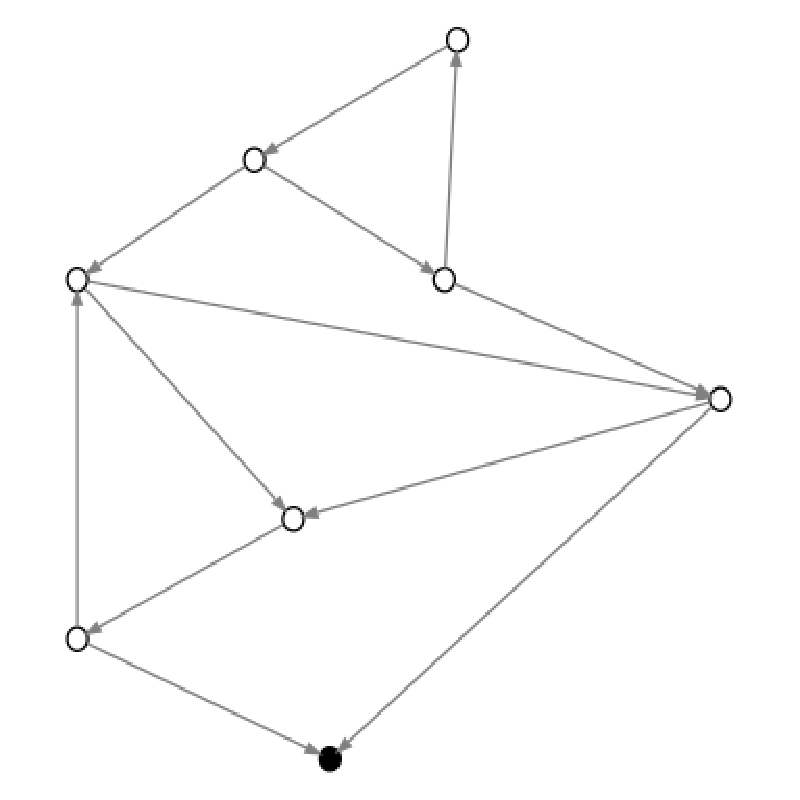
\includegraphics[scale=0.8]{images/applicationOfPrinterPipeFilterOnTarjanModel-phase-PrinterPipeFilter-level-0.eps}
  \caption{Rappresentazione di un modello SBML mediante un grafo}
  \label{fig:simple-black-and-white}
\end{figure}

La Figura \ref{fig:simple-black-and-white} riporta il risultato di
questa funzionalit\`a applicata ad un modello SBML codificato in un
grafo.

\subsection{Applicare la visita in profondit\`a}
Con questa funzionalit\`a si vuole visitare in profondit\`a il grafo
in input.

Il risultato prodotto \`e una foresta di alberi \emph{DFS}, i cui
archi sono un sotto insieme dell'insieme di archi del grafo originale,
attraversati durante la computazione.

Inoltre siamo interessati ad associare, per ogni vertice, una coppia
di interi che indica il momento in cui la visita esplora un vertice e
quando l'esplorazione del vicinato di tale vertice viene
completata. Queste informazioni possono risultare molto utili in fase
di studio del grafo; abbiamo ripreso questo spunto da
\cite{Algorithms}.

Vediamo i risultati di una sua esecuzione, dopo aver composto la
funzionalit\`a descritta nella Sezione
\ref{subsection:represent-it-in-black-and-white}. La Figura
\ref{fig:before-applying-dfs-search} riporta il grafo originale di
partenza, preso da \cite{Algorithms}:
\begin{figure}
  \centering
  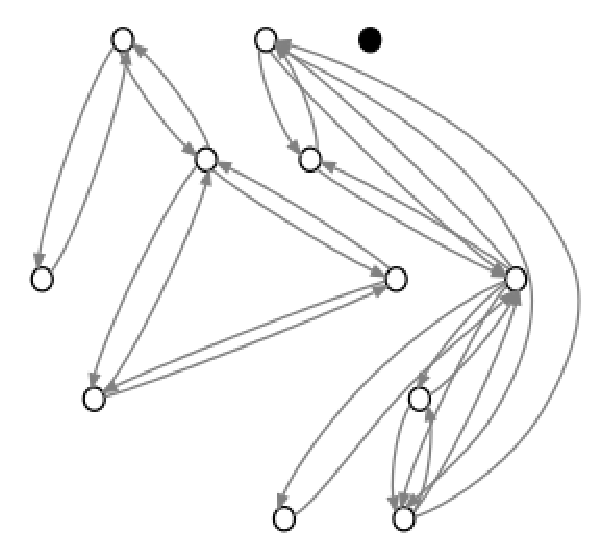
\includegraphics{images/OnePipingLevelUnitTest_Printer_DFS_PrinterPipe_Papadimitriou-phase-PrinterPipeFilter-level-0.eps}
  \caption{Grafo che si vuole visitare}
  \label{fig:before-applying-dfs-search}
\end{figure}
visitandolo in profondit\`a otteniamo la foresta di alberi \emph{DFS}
riportata in Figura \ref{fig:dfs-forest}.
\begin{figure}
  \centering
  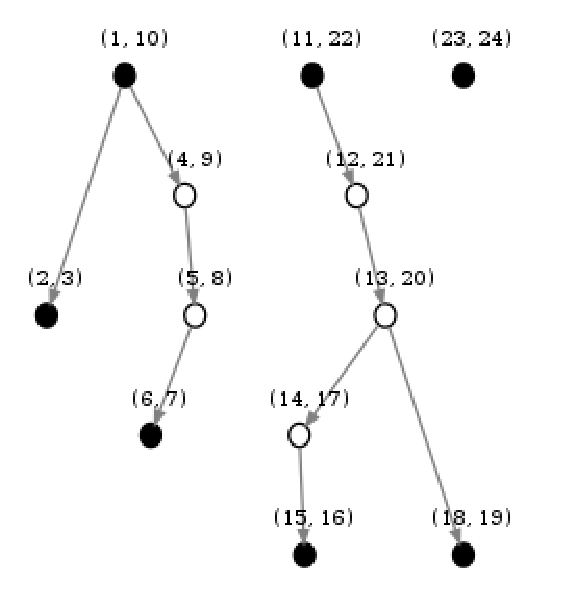
\includegraphics{images/OnePipingLevelUnitTest_Printer_DFS_PrinterPipe_Papadimitriou-phase-PrinterPipeFilter-level-2.eps}
  \caption{Risultato della visita in profondit\`a del grafo riportato
    in Figura \ref{fig:before-applying-dfs-search}}
  \label{fig:dfs-forest}
\end{figure}

\subsection{Applicare l'algoritmo di Tarjan}
\label{subsection:use-case-tarjan}
Con questa funzionalit\`a si vuole applicare l'algoritmo di Tarjan per
la ricerca delle componenti fortemente connesse al grafo in input.

Il risultato prodotto \`e un grafo che ha come nodi le componenti
fortemente connesse e come archi la relazione di vicinato tra le
componenti.

Inoltre siamo interessati ad associare, per ogni vertice, un intero
che indica la cardinalit\`a della componente fortemente connessa che
esso rappresenta.

Vediamo i risultati di una sua esecuzione, dopo aver composto la
funzionalit\`a descritta nella precedente Sezione
\ref{subsection:represent-it-in-black-and-white}: la Figura
\ref{fig:before-applying-tarjan} riporta il grafo originale di
partenza, preso da \cite{Algoritmica}:
\begin{figure}
  \centering
  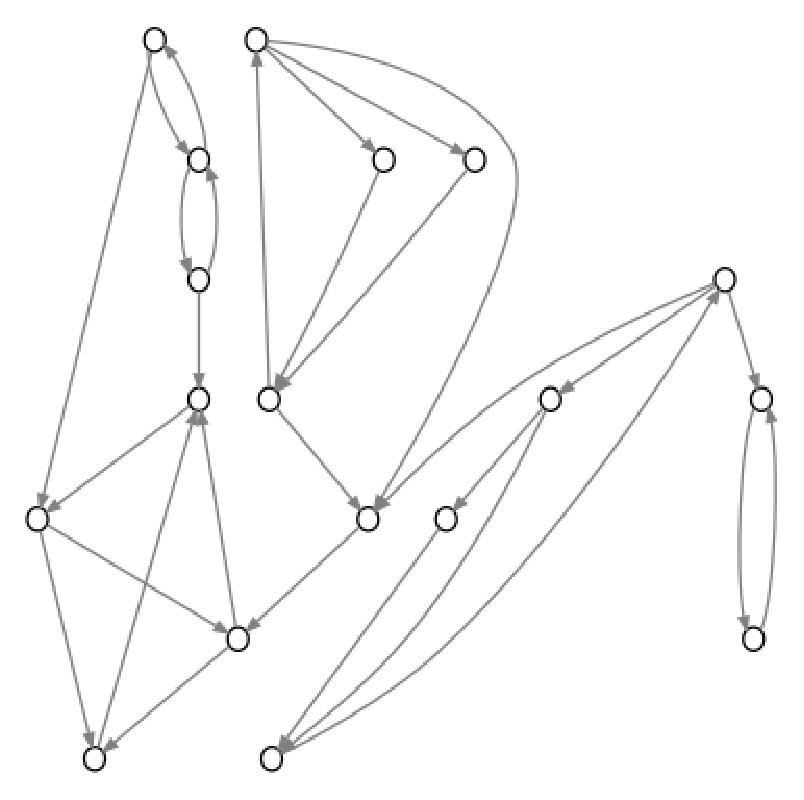
\includegraphics{images/OnePipingLevelUnitTest_Printer_DFS_PrinterPipe_Crescenzi-phase-PrinterPipeFilter-level-0.eps}
  \caption{Grafo di cui si vuole ricercare le componenti fortemente
    connesse}
  \label{fig:before-applying-tarjan}
\end{figure}
applicando l'algoritmo di Tarjan a tale grafo otteniamo la
minimizzazione riportata in Figura \ref{fig:tarjan-output}.
\begin{figure}
  \centering
  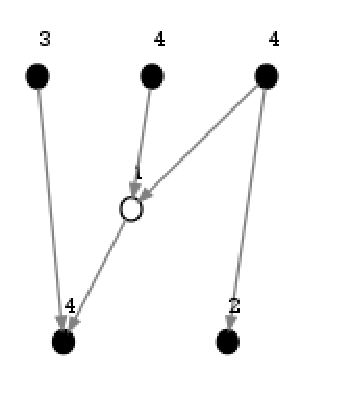
\includegraphics{images/OnePipingLevelUnitTest_Printer_DFS_PrinterPipe_Crescenzi-phase-PrinterPipeFilter-level-2.eps}
  \caption{Componenti fortemente connesse del grafo riportato in
    Figura \ref{fig:before-applying-tarjan}}
  \label{fig:tarjan-output}
\end{figure}

\subsection{Rappresentazione tabulare}
Con questa funzionalit\`a si vuole rappresentare il grafo in input in
formato testuale, usando uno schema tabellare.

Il \emph{side-effect} prodotto \`e collezionare le informazioni
richieste visitando il grafo e scriverle in un file dedicato.

Inoltre, per comodit\`a, vogliamo comporre pi\`u di una funzionalit\`a
ed avere le informazioni relative alle computazioni di ognuna,
presenti nello stesso documento.

Vediamo i risultati di una sua esecuzione, allegando un documento
prodotto:
\begin{lstlisting}
phase-PlainTextStatsPipeFilter-level-2
NOfVertices: 1
	NOfComponents:	206
	NOfEdges:	183
	NOfSources:	108
	NOfSinks:	96
	NOfWhites:	2

NOfVertices: 2
	NOfComponents:	9
	NOfEdges:	1
	NOfSources:	1
	NOfSinks:	8
	NOfWhites:	0

NOfVertices: 3
	NOfComponents:	5
	NOfEdges:	0
	NOfSources:	0
	NOfSinks:	5
	NOfWhites:	0

NOfVertices: 4
	NOfComponents:	1
	NOfEdges:	0
	NOfSources:	0
	NOfSinks:	1
	NOfWhites:	0

NOfVertices: 396
	NOfComponents:	1
	NOfEdges:	89
	NOfSources:	0
	NOfSinks:	0
	NOfWhites:	1

phase-PlainTextStatsPipeFilter-level-0
	NOfVertices:	639
	NOfEdges:	2209
	NOfSources:	108
	NOfSinks:	95
	NOfWhites:	436

\end{lstlisting}
Questo output necessita di alcune spiegazioni. Quello riportato \`e il
documento che viene generato da questa funzionalit\`a, collezionando
in un primo momento le informazioni sul grafo originale (riportate
sotto l'etichetta \emph{phase-PlainTextStatsPipeFilter-level-0}) e in
un secondo momento, dopo aver applicato l'algoritmo di Tarjan, le
informazioni sul grafo minimizzato (riportate sotto l'etichetta
\emph{phase-PlainTextStatsPipeFilter-level-2}).

Come si nota i formati delle rappresentazioni tabulari sono vicini ma
non identici. Dato il seguente blocco relativo al primo passo:
\begin{lstlisting}
phase-identifier
	NOfVertices:	v
	NOfEdges:	e
	NOfSources:	s
	NOfSinks:	d
	NOfWhites:	w
\end{lstlisting}
allora il grafo in input $G = (V, E)$, al passo
\emph{phase-identifier}, \`e tale che $|E| = e$ e $|V| = v$, di cui
$s$ vertici sono sorgenti, $d$ vertici sono pozzi e $w (= v -s -d)$
sono intermedi.

Definiamo adesso la semantica associata alle informazioni collezionate
per il secondo passo. Come si pu\`o notare, queste informazioni
ripetono uno schema, del quale \`e sufficiente dare la semantica,
quante volte \`e necessario per elencare tutti i dati raccolti. Sia
dato il \emph{template}:
\begin{lstlisting}
NOfVertices: v
	NOfComponents:	c
	NOfEdges:	e
	NOfSources:	s
	NOfSinks:	d
	NOfWhites:	w  
\end{lstlisting}
allora nel grafo minimizzato esistono $c$ componenti fortemente
connesse, ognuna delle quali raggruppa $v$ vertici. Esistono $e$ archi
uscenti in totale dalle $c$ componenti e queste sono partizionate in
$s$ componenti sorgenti, $d$ componenti pozzo e $w$ componenti
intermedie.

Come abbiamo detto ad inizio sezione, questa funzionalit\`a non
trasforma il grafo in input, anzi \`e ortogonale ad un'intera
composizione di funzionalit\`a in quanto, elencando i dati raccolti
per ogni specifico \emph{phase-identifier}, non ha dipendenze da
ognuna di esse.

\subsection{Ridurre la complessit\`a collassando i nodi sorgente}
Con questa funzionalit\`a si vuole eliminare tutti i vertici sorgenti
contenuti nel grafo in input, introducendo al loro posto un nuovo
vertice sorgente, tale che il suo vicinato sia uguale all'unione dei
vicinati dei vertici rimossi.

Vediamo i risultati di una sua esecuzione, applicando la
minimizzazione al grafo di input, dopo aver composto la funzionalit\`a
descritta nella precedente Sezione
\ref{subsection:represent-it-in-black-and-white}:
\begin{lstlisting}
phase-PlainTextStatsPipeFilter-level-1
	NOfVertices:	386
	NOfEdges:	1339
	NOfSources:	1
	NOfSinks:	85
	NOfWhites:	300
\end{lstlisting}
Come si vede dalle informazioni riportate, il nuovo grafo, input per
successive computazioni, ha un solo vertice sorgente.

\subsection{Indagare propriet\`a di una batteria di modelli}
\label{subsection:use-case-result-viewer}
Con questa funzionalit\`a si vuole rappresentare informazioni relative
ad una batteria di modelli, dei quali abbiamo calcolato le componenti
fortemente connesse, attraverso una semplice GUI utilizzando il
framework \emph{SWING}.

In realt\`a quello che ci piacerebbe costruire \`e un visualizzatore
di strutture dati, costruite appositamente per contenere le
informazioni di interesse, senza essere dipendenti dal risultato di
una computazione appena conclusa. Ovvero, vorremmo serializzare tale
struttura dati in una path del file system e poterla visualizzare
successivamente. Questo secondo noi \`e un approccio pi\`u modulare in
quanto permette di creare strutture dati e poterle scambiare,
utilizzando la maschera come semplice \emph{render}, anche se non
abbiamo generato noi stessi la serializzazione delle informazioni.

Inoltre siamo interessati a condurre la nostra indagine restringendosi
non solo ad un modello (e quindi ad un solo grafo), bensi vorremmo
analizzare un insieme di modelli affinch\`e sia possibile studiare in
che tipo di componente fortemente connessa ogni metabolito incontrato
appare.

\begin{figure}
  \centering
  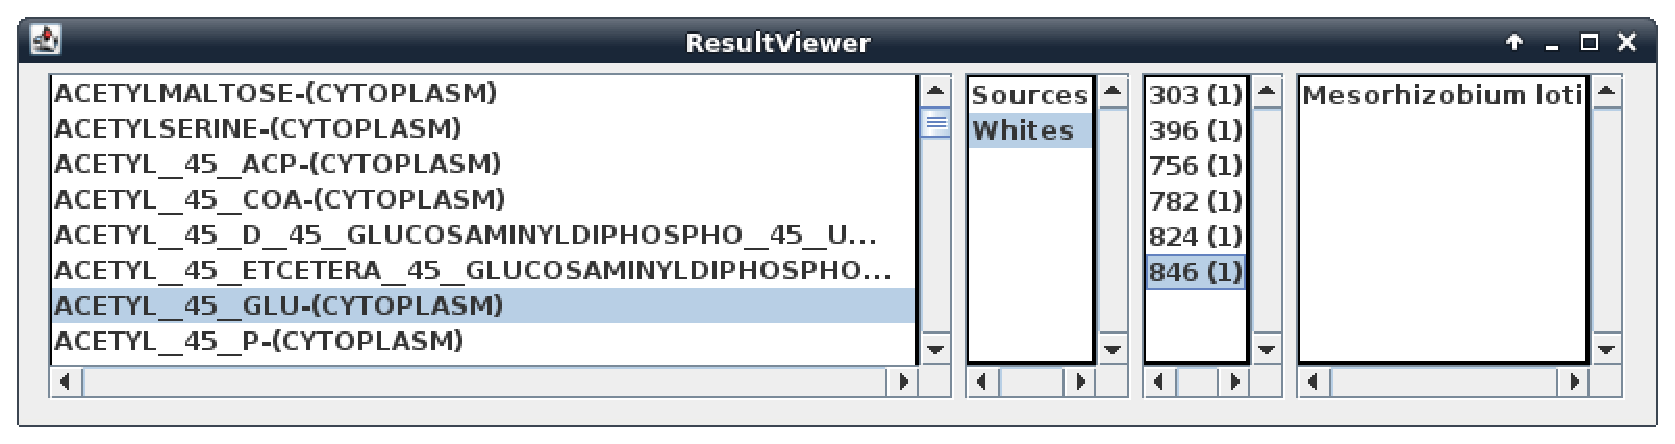
\includegraphics[scale=.5,
  angle=90]{images/ResultViewer-execution.eps}
  \caption{Visualizzatore dell'indagine relativa ad un insieme di
    modelli}
  \label{fig:result-viewer-scc}
\end{figure}
La Figura \ref{fig:result-viewer-scc} riporta uno screenshot, diamo
adesso la semantica delle informazioni rappresentate nella maschera.

Il frame contiene i seguenti componenti, che andiamo a descrivere
seguendo l'ordine da sinistra verso destra e dall'alto verso il basso:
\begin{itemize}
\item una tabella dove vengono elencati tutti i modelli che sono stati
  oggetto di indagine. Per ogni modello si associano tre coppie $(c,
  v)$ per tre colonne, ognuna rappresentante una tipologia di vertice
  (\emph{sources, whites, sinks}). Per esempio, se una coppia $c, v$
  appartiene alla riga del modello $m$ e alla colonna $whites$, allora
  significa che nel modello $m$ esistono $c$ componenti fortemente
  connesse di tipo $whites$, le quali contengono in totale $m$ vertici
  (che di conseguenza hanno pure loro il ruolo di $whites$);
\item una \emph{list-box} nella quale sono riportate delle
  informazioni relative ai metaboliti. Ogni oggetto raggruppa i
  metaboliti in base ai ruoli (ovvero in base alla tipologia di
  vertice) che hanno in tutti i modelli analizzati.

  Inoltre si calcola anche una loro frequenza in percentuale per avere
  un raffronto immediato riguardo alla predominanza dei ruoli svolti:
  si considerano tutte le possibili combinazioni dell'insieme
  ${sources, whites, sinks}$, escludendo l'insieme vuoto;
\item nella successiva \emph{list-box} vengono elencate tutte i
  metaboliti contenuti in almeno uno dei modelli oggetto
  dell'indagine. Ogni metabolito \`e codificato con una stringa
  composta dall'identificatore e, tra parantesi tonde, il nome del
  compartimento in cui risiede;
\item cliccando su un metabolito $s$, nella successiva \emph{list-box}
  vengono elencati i tipi delle componenti fortemente connesse che
  contengono il metabolito $s$;
\item cliccando su una tipologia $t$ di componente fortemente
  connessa, nella successiva \emph{list-box} vengono elencate le
  cardinalit\`a delle componenti fortemente connesse che contengono il
  metabolito $s$ e sono di tipologia $t$. Ad ogni cardinalit\`a si
  concatena un numero intero che indica la cardinalit\`a dell'insieme
  rappresentato nell'ultima \emph{list-box}, che descriveremo nel
  prossimo punto;
\item cliccando su una cardinalit\`a $c$, nell'ultima \emph{list-box}
  vengono elencati i modelli, la cui applicazione dell'algoritmo di
  Tarjan, ha prodotto un grafo in cui esiste una componente fortemente
  connessa tale che contiene il metabolito $s$, \`e di tipo $t$ ed ha
  una cardinalit\`a $c$.
\end{itemize}

Non solo le ultime quattro \emph{list-box} sono contestualmente
correlate, ma anche la tabella e la \emph{list-box} con le
informazioni per tipologia di vertice lo sono. In particolare,
selezionando nella tabella una o pi\`u righe, nella \emph{list-box}
\`e possibile avere le informazioni riguardo ai metaboliti contenuti
nei modelli selezionati. Se la selezione \`e vuota, allora le
informazioni sono relative a tutti i modelli.

Inoltre abbiamo esteso queste correlazioni anche tra il percorso
selezionato nelle ultime quattro \emph{list-box} e la tabella (e di
conseguenza alla prima \emph{list-box}). Selezionando un metabolito
dalla seconda \emph{list-box} vengono selezionati in automatico nella
tabella tutti i modelli che lo contengono e, come spiegato nel
paragrafo precedente, anche la \emph{list-box} contenente le
informazioni per tipologia di vertice verr\`a aggiornata di
conseguenza.

Se si raffina il percorso, ad esempio scegliendo la tipologia di
vertice e la cardinalit\`a nelle rispettive \emph{list-box}, viene
raffinata la selezione nella tabella dei modelli.

\subsection{Analizzare un grafo non associato ad un modello SBML}
Nelle precedenti sezioni abbiamo sempre assunto di lavorare su un
modello metabolico, ma niente ci vieta di poter utilizzare la libreria
su un grafo arbitrario che costruiamo direttamente utilizzando oggetti
del nostro modello dati.

Questo rende la libreria non strettamente legata ai concetti nel campo
della biologia e, in particolare, delle reti metaboliche, restando
invece aperta ad utilizzi nel campo della teoria dei grafi (in
realt\`a il grafo riportato in Figura \ref{fig:simple-black-and-white}
non \`e altro che il grafo utilizzato da Tarjan nel suo articolo
\footnote{aggiungere qui riferimento bibliografico all'articolo di
  Tarjan sull'algoritmo per le componenti fortemente connesse}).


